\documentclass[aspectratio=169,11pt]{beamer}

\usepackage[T1]{fontenc}
\usepackage[utf8]{inputenc}
\usepackage{lmodern}
\usepackage{booktabs,amsmath,amssymb}
\usepackage{tikz}
\usepackage{pgfpages}
\usepackage{qrcode}

% --------------------------------------------------------------------
\usepackage{amsmath}

\newcommand{\rel}[1]{\mathrel{#1}}

% --------------------------------------------------------------------
\newenvironment{tightcenter}{%
  \setlength\topsep{0pt}
  \setlength\parskip{0pt}
  \begin{center}}
{\end{center}}

% --------------------------------------------------------------------
% Acronyms, names, ...

\usepackage{xspace}

\def\EasyCrypt{\textsc{EasyCrypt}\xspace}
\def\prhl{\textsc{pRHL}\xspace}
\def\phl{\textsc{pHL}\xspace}
\def\hl{\textsc{HL}\xspace}
\def\al{\textsc{AL}\xspace}
\newcommand{\WhyThree}{\textsf{Why3}\xspace}

% --------------------------------------------------------------------
% Inference rules
\usepackage{ec/mathpartir}

\newenvironment{cmathpar}
{\begin{tightcenter}\begin{mathpar}}
{\end{mathpar}\end{tightcenter}}

% --------------------------------------------------------------------
% EasyCrypt listings

\usepackage{textcomp}
\usepackage{listings}

\newcommand{\ensuretext}[1]{\ensuremath{\text{#1}}}

\input{ec/easycrypt.lst}

\lstnewenvironment{easycrypt}[3][]%
  {\lstset{language=easycrypt,caption={#2},label={#3},#1}}%
  {}

\lstnewenvironment{easycryptfloat}[3][]%
  {\lstset{language=easycrypt,float=tp,caption={#2},label={#3},#1}}%
  {}

\newcommand{\ecinput}[2][]%
{\lstinputlisting[language=easycrypt,#1]{#2}}

\newcommand{\ecinputfloat}[1]%
{\lstinputlisting[language=easycrypt,float=tp]{#1}}

\def\ls{\lstinline}
\def\ec#1{\lstinline[language=easycrypt-math]"#1"}
\def\ecn#1{\lstinline[language=easycrypt-math-nocolors]"#1"}

\def\Arg{\ensuretext{\ec{arg}}}

% --------------------------------------------------------------------
% Typesetting judgments
\newcommand{\pRHL}[4]{\{#1\}\; #2 \mathrel{\sim} #3\; \{#4\}}
\newcommand{\pHL}[5]{\{#1\}\; #2\; \{#3\} \mathrel{#4} #5}
\newcommand{\HL}[3]{\{#1\}\; #2\; \{#3\}}
\newcommand{\PR}[4]{\mathbf{Pr} [#3, #1(#2) : #4]}

\newcommand{\pRHLs}[4]{\ec{equiv [#2 ~ #3: #1 ==> #4]}}
\newcommand{\pHLs}[5]{\ec{phoare [#2: #1 ==> #3] #4 #5}}
\newcommand{\HLs}[3]{\ec{hoare [#2: #1 ==> #3]}}
\newcommand{\PRs}[4]{\ec{Pr[#1(#2) @ &#3: #4]}}

% --------------------------------------------------------------------
\newcommand{\mem}[1]{#1}
\newcommand{\inmem}[2]{#1\langle{#2}\rangle}
\newcommand{\backticksym}{\symbol{'096}} % produces `

\usepackage{xspace}

\newcommand{\xmss}{\ensuremath{\mathrm{XMSS}}\xspace}
\newcommand{\xmssmt}{\ensuremath{\mathrm{XMSS}^{\mathrm{MT}}}\xspace}
\newcommand{\wots}{\ensuremath{\mathrm{WOTS}^{+}}\xspace}


\usetikzlibrary{arrows.meta,positioning,calc,fit}

\hypersetup{
  pdfauthor={Manuel Barbosa, François Dupressoir,
    Rui Fernandes, Andreas Hülsing, Matthias Meijers,
  Pierre-Yves Strub},
  pdftitle={Completing the Chain: Verified Implementations of
  Hash-Based Signatures and Their Security}
}

\definecolor{Navy}{HTML}{102C46}
\definecolor{Teal}{HTML}{00877E}
\definecolor{Gold}{HTML}{B96A16}
\definecolor{Mist}{HTML}{EDF4F6}
\definecolor{Muted}{HTML}{526575}

\hypersetup{colorlinks=true,urlcolor=Teal,linkcolor=Navy,citecolor=Teal}

\setbeamercolor{normal text}{fg=Navy,bg=white}
\setbeamercolor{frametitle}{fg=Navy}
\setbeamercolor{structure}{fg=Teal}
\setbeamercolor{alerted text}{fg=Gold}
\setbeamercolor{block title}{fg=white,bg=Teal}
\setbeamercolor{block body}{fg=Navy,bg=Mist}
\setbeamerfont{frametitle}{size=\Large,series=\bfseries}
\setbeamerfont{title}{size=\LARGE,series=\bfseries}
\setbeamertemplate{navigation symbols}{}
\setbeamertemplate{itemize items}[circle]
\setbeamersize{text margin left=8mm,text margin right=8mm}
\setbeamertemplate{frametitle}{\vspace{4mm}\insertframetitle\par\vspace{1mm}}
\setbeamertemplate{footline}{\hfill\scriptsize\color{Muted}%
\insertframenumber\hspace{8mm}\vspace{3mm}}

\title{Completing the Chain:}
\subtitle{Verified Implementations of Hash-Based Signatures\\and Their Security}
\author{Manuel Barbosa \and François Dupressoir \and \textbf{Rui
Fernandes}\\ Andreas H\"ulsing \and Matthias Meijers \and Pierre-Yves Strub}
\date{CHES 2026}

\begin{document}

\begin{frame}[plain]
  \begin{tikzpicture}[remember picture,overlay]
    \node[anchor=north east,inner sep=0] at
    ([xshift=-8mm,yshift=-5mm]current page.north east) {%
    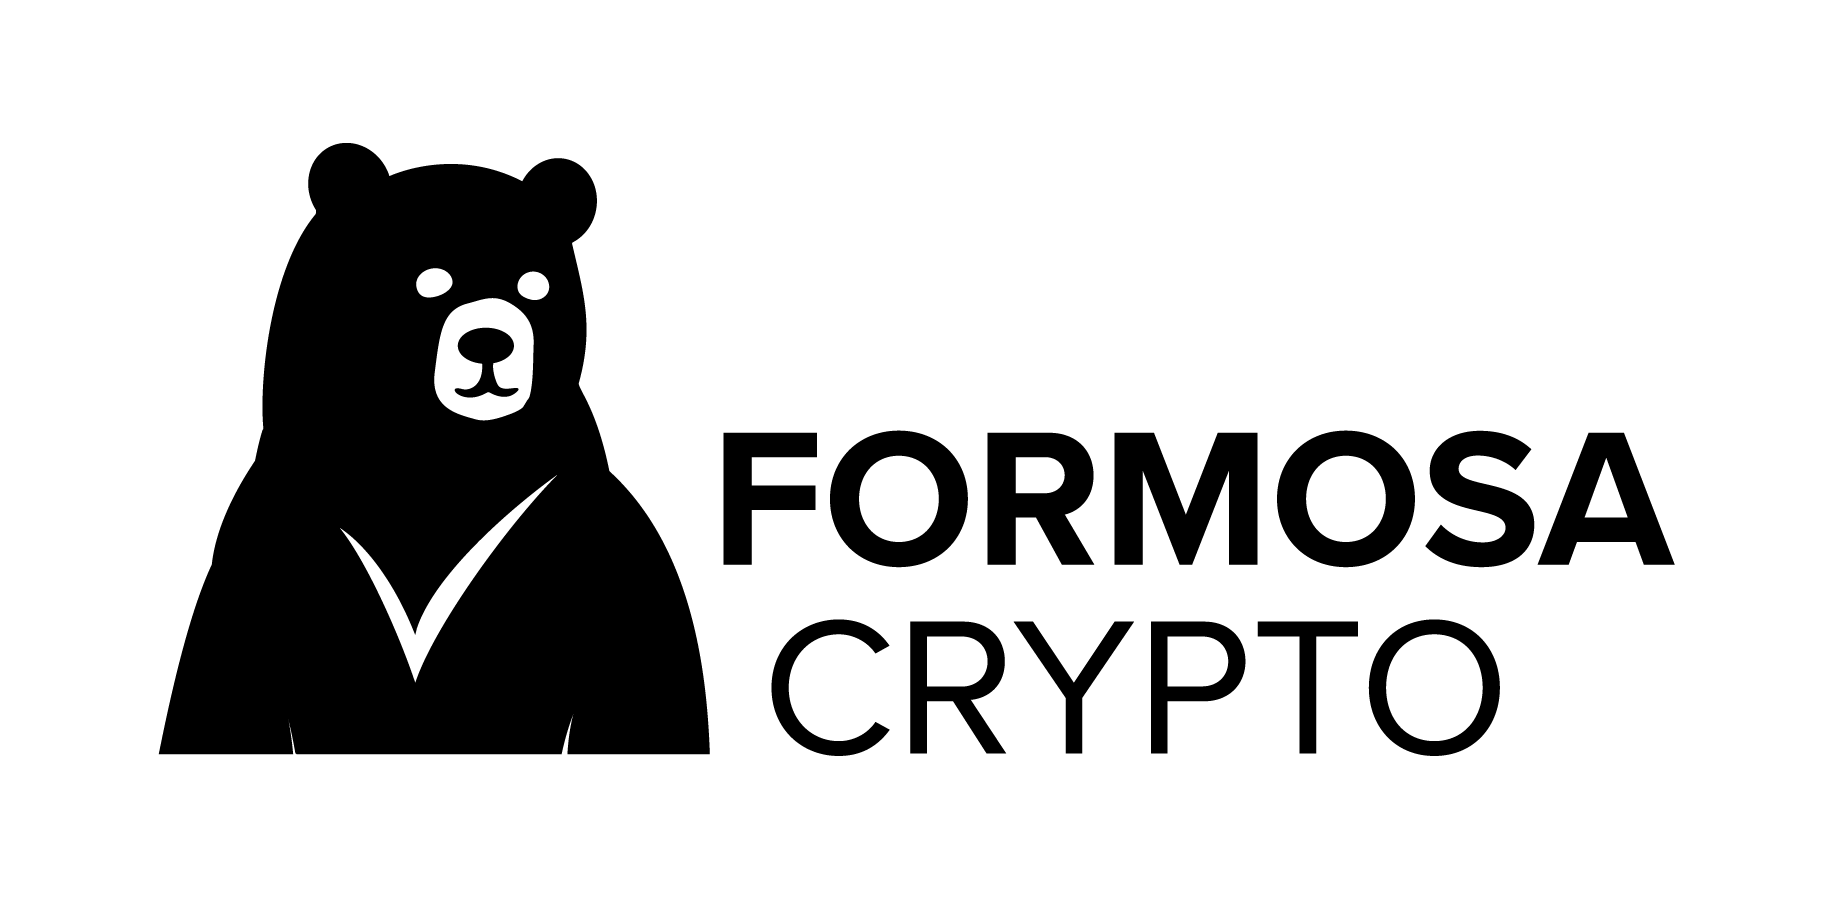
\includegraphics[width=30mm]{img/formosa.png}};
    \node[anchor=south east,inner sep=0] at
    ([xshift=-8mm,yshift=18mm]current page.south east) {%
      \begin{minipage}{49mm}
        \centering
        \begin{minipage}{23mm}
          \centering
          {\hypersetup{urlcolor=black}\color{black}\qrcode[height=19mm,level=M]{https://github.com/formosa-crypto/formosa-xmss}}\par\vspace{2mm}
          {\scriptsize\color{Muted}GitHub Repository}
        \end{minipage}\hfill
        \begin{minipage}{23mm}
          \centering
          {\hypersetup{urlcolor=black}\color{black}\qrcode[height=19mm,level=M]{https://doi.org/10.46586/tches.v2026.i3.958-981}}\par\vspace{2mm}
          {\scriptsize\color{Muted}Paper}
        \end{minipage}
    \end{minipage}};
  \end{tikzpicture}%
  \vspace{5mm}
  {\color{Teal}\small 11B: Implementation Tools \& Formal
  Verification}\par\vspace{4mm}
  {\usebeamerfont{title}\inserttitle\par}\vspace{3mm}
  {\large\insertsubtitle\par}\vspace{7mm}
  {\small\insertauthor\par}\vspace{5mm}
  {\small\insertinstitute\par}\vfill\vspace{10mm}
  {\small\color{Muted}CHES 2026\hfill}
\end{frame}

% XMSS key generation: RFC 8391, Section 4.1.7.
% Local overlay styles keep the diagram geometry fixed between steps.
\tikzset{
  xmss hidden/.style={opacity=0,text opacity=0},
  xmss show/.code args={<#1>}{\alt<#1>{}{\pgfkeysalso{xmss hidden}}},
  xmss node/.style={circle,draw=Teal,fill=Mist,minimum size=5mm,
    inner sep=0pt}
}

% Example tree with height h=3.
\newcommand{\xmsskeygentree}{%
  \begin{tikzpicture}[x=0.68cm,y=0.68cm,font=\scriptsize,>=Latex]
    \foreach \i in {0,...,7} {
      \node[xmss node]
        (l\i) at (\i,0) {};
      % Two vertically separated keys represent the secret/public keypair.
      \begin{scope}[shift={(\i,-1.35)},draw=Gold,line width=0.7pt]
        \foreach \keyheight in {-0.16,0.16} {
          \draw (-0.15,\keyheight) circle[radius=0.075cm];
          \draw (-0.04,\keyheight) -- (0.22,\keyheight);
          \draw (0.13,\keyheight) -- (0.13,\keyheight-0.10);
          \draw (0.22,\keyheight) -- (0.22,\keyheight-0.10);
        }
      \end{scope}
      \draw[->,Teal] (\i,-1.05) --
        node[midway,right,rotate=90,anchor=south,font=\tiny] {LTree}
        (l\i.south);
    }
    \node[text=Gold] at (3.5,-1.95) {\wots keypairs};
    \foreach \i/\x in {0/0.5,1/2.5,2/4.5,3/6.5} {
      \node[xmss node] (p\i) at (\x,1) {};
      \pgfmathtruncatemacro{\leftleaf}{2*\i}
      \pgfmathtruncatemacro{\rightleaf}{2*\i+1}
      \draw[Muted] (p\i) -- (l\leftleaf);
      \draw[Muted] (p\i) -- (l\rightleaf);
    }
    \node[xmss node] (q0) at (1.5,2) {};
    \node[xmss node] (q1) at (5.5,2) {};
    \foreach \parent/\child in {q0/p0,q0/p1,q1/p2,q1/p3}
      \draw[Muted] (\parent) -- (\child);
    \node[xmss node,label=above:{public root}]
      (r) at (3.5,3) {};
    \foreach \child in {q0,q1}
      \draw[Muted] (r) -- (\child);
  \end{tikzpicture}%
}

\begin{frame}{XMSS: Overview}
  \begin{itemize}
    \setlength{\itemsep}{4mm}
    \item XMSS~\cite{DBLP:conf/pqcrypto/BuchmannDH11} is a stateful hash-based signature scheme.
    \item Security relies on the security of the underlying hash function.
    \item XMSS combines a one-time signature scheme (\wots) with a Merkle tree.
    \vspace{2mm}
    \begin{itemize}
      \setlength{\itemsep}{1mm}
      \item The root of the Merkle tree is the public key of the XMSS instance.
      \item Each leaf corresponds to a (compressed) \wots public key.
      \item A Merkle tree of height $h$ has $2^h$ leaves, and thus allows $2^h$ signing $2^h$ messages.
    \end{itemize}
  \end{itemize}
\end{frame}

% \wots key generation and signing: RFC 8391, Sections 3.1.3--3.1.5.
\begin{frame}{\wots: Key Generation}
  \small
  \begin{enumerate}
    \setlength{\itemsep}{2mm}
    \item Generate $\ell$ secret $n$-byte values
      $\mathsf{sk}_0,\ldots,\mathsf{sk}_{\ell-1}$ (randomly or pseudorandomly).
    \item Each value starts a hash chain: apply $w-1$ steps to obtain
      $\mathsf{pk}_j=\mathsf{chain}(\mathsf{sk}_j,0,w-1)$.
    \item The \wots public key is the array of all $\ell$ chain endpoints.
  \end{enumerate}
  \vspace{2mm}
  \begin{center}
    \begin{tikzpicture}[x=1.7cm,y=0.75cm,font=\scriptsize,>=Latex]
      \foreach \j/\y in {0/1,1/0,\ell-1/-1} {
        \node[anchor=east,text=Gold] at (-0.3,\y) {$\mathsf{sk}_{\j}$};
        \foreach \k in {0,...,3}
          \node[xmss node] (k\y\k) at (\k,\y) {};
        \foreach \k/\next in {0/1,1/2,2/3}
          \draw[->,Teal] (k\y\k) -- (k\y\next);
        \node[anchor=west,text=Teal] at (3.3,\y) {$\mathsf{pk}_{\j}$};
      }
      \node at (1.5,-1.65) {Example: $w=4$, three steps per chain (selected chains shown).};
    \end{tikzpicture}
  \end{center}
  {\footnotesize
    $n$: element size in bytes; $w$: Winternitz parameter;
    $\ell$: number of message and checksum digits.\\[1mm]
    Each step uses a hash key and bitmask derived from public
    $\mathsf{SEED}$ and the keypair, chain, and step address.
  }
\end{frame}

\begin{frame}{\wots: Signature Generation}
  \small
  \begin{enumerate}
    \setlength{\itemsep}{2mm}
    \item Encode the $n$-byte message digest $D$ as base-$w$ digits
      $m_0,\ldots,m_{\ell_1-1}$.
    \item Append the base-$w$ digits of the checksum
      $C=\sum_{j=0}^{\ell_1-1}(w-1-m_j)$,
      giving $\ell$ digits $a_j\in\{0,\ldots,w-1\}$.
    \item Reveal one node per chain:
      $\sigma_j=\mathsf{chain}(\mathsf{sk}_j,0,a_j)$.
      The signature is $(\sigma_0,\ldots,\sigma_{\ell-1})$.
  \end{enumerate}
  \vspace{2mm}
  \begin{center}
    \begin{tikzpicture}[x=1.7cm,y=0.75cm,font=\scriptsize,>=Latex]
      \foreach \j/\y/\digit in {0/1/1,1/0/3,2/-1/2} {
        \node[anchor=east] at (-0.3,\y) {$a_{\j}=\digit$};
        \foreach \k in {0,...,3}
          \node[xmss node,draw=Muted,fill=white] (s\j\k) at (\k,\y) {};
        \foreach \k/\next in {0/1,1/2,2/3} {
          \ifnum\k<\digit
            \draw[->,Teal,thick] (s\j\k) -- (s\j\next);
          \else
            \draw[->,Muted,dashed] (s\j\k) -- (s\j\next);
          \fi
        }
        \node[xmss node,draw=Gold,fill=Gold!20] at (s\j\digit) {};
        \node[anchor=west,text=Gold] at (3.3,\y) {$\sigma_{\j}$: step $\digit$};
      }
      \node at (1.5,-1.65) {Example: $w=4$; gold nodes form the signature (selected chains shown).};
    \end{tikzpicture}
  \end{center}
  {\footnotesize
    Verification completes each chain with $w-1-a_j$ steps to recover its endpoint.\\[1mm]
    \alert{Each \wots keypair signs at most one message digest.}
  }
\end{frame}

\begin{frame}{XMSS: Key Generation}
  \small
  \setbeamerfont{itemize/enumerate body}{size=\small}
  \begin{columns}[T,onlytextwidth]
    \begin{column}{0.54\textwidth}
      \begin{enumerate}
        \item Start from $2^h$ \wots keypairs: one for each leaf
          of the tree.
        \item Compress each \wots public key via an L-tree
          (LTree) to an $n$-byte value. These values are the leaves.
        \item Hash pairs of nodes upward, level by level,
          to obtain the $n$-byte root.
      \end{enumerate}
      {\setbeamerfont{block title}{size=\small}
        \setbeamerfont{block body}{size=\footnotesize}
        \begin{block}{Scheme parameters}
          $h$: tree height ($2^h$ leaves).\\
          $n$: hash output length in bytes.
        \end{block}
}
    \end{column}
    \begin{column}{0.43\textwidth}
      \centering
      \vspace{3mm}
      \xmsskeygentree\\[3mm]
      \small Example: $h=3$

    \end{column}
  \end{columns}
  \vspace{0mm}
  {\footnotesize
    \textbf{Public key:} $\mathsf{PK}=(\mathsf{root},\mathsf{SEED})$, with public seed $\mathsf{SEED}$.\\
    \textbf{Secret key:} $\mathsf{SK}=(i,\{\mathsf{sk}^{\mathrm{\wots}}_j\}_{j=0}^{2^h-1},\mathsf{SK}_{\mathrm{PRF}},\mathsf{PK})$.\\
    $\mathsf{SK}_{\mathrm{PRF}}$: secret key for message randomization.
  }
\end{frame}

\begin{frame}{\xmss: Signature Verification}
  \relax
  {\small
    \textbf{Inputs}: message $M$, $\mathsf{PK}=(\mathsf{root},\mathsf{SEED})$,
    $\sigma=(i,R,\sigma_{\mathrm{\wots}},\mathsf{auth}_i)$, with $0\leq i<2^h$.\par}
  \vspace{2mm}
  \begin{columns}[T,onlytextwidth]
    \begin{column}{0.54\textwidth}
      \begin{enumerate}
        \small
        \setlength{\itemsep}{0.5mm}
        \item<1-> Recompute the message digest $D = H_{\mathrm{msg}}(R\mathbin\Vert\mathsf{root}\mathbin\Vert i,M)$.
        \item<2-> Complete the \wots chains from
          $\sigma_{\mathrm{\wots}}$ to recover $\mathsf{pk}_i$.
        \item<3->LTree compression gives leaf $i$.
        \item<4-> Hash upward with the $h$ authentication siblings.
          Bits of $i$ determine left/right order.
        \item<5-> Accept if the reconstructed root equals
          $\mathsf{root}$ in the public key.
      \end{enumerate}
    \end{column}
    \begin{column}{0.43\textwidth}
      \centering
      \vspace{2mm}
      \begin{tikzpicture}[x=0.68cm,y=0.7cm,font=\scriptsize]
        \foreach \i in {0,...,7}
          \node[xmss node,draw=Muted!45,fill=white] (v\i) at (\i,0) {};
        \foreach \i/\x in {0/0.5,1/2.5,2/4.5,3/6.5} {
          \node[xmss node,draw=Muted!45,fill=white] (p\i) at (\x,1) {};
          \pgfmathtruncatemacro{\leftleaf}{2*\i}
          \pgfmathtruncatemacro{\rightleaf}{2*\i+1}
          \draw[Muted!40] (p\i) -- (v\leftleaf);
          \draw[Muted!40] (p\i) -- (v\rightleaf);
        }
        \node[xmss node,draw=Muted!45,fill=white] (q0) at (1.5,2) {};
        \node[xmss node,draw=Muted!45,fill=white] (q1) at (5.5,2) {};
        \node[xmss node,draw=Muted!45,fill=white,label=above:{public root}]
          (r) at (3.5,3) {};
        \foreach \parent/\child in {q0/p0,q0/p1,q1/p2,q1/p3,r/q0,r/q1}
          \draw[Muted!40] (\parent) -- (\child);
        \foreach \name in {v3,p0,q1}
          \node[xmss node,draw=Gold,fill=Gold!20] at (\name) {};
        \foreach \name/\step in {v2/2,p1/3,q0/4,r/5}
          \node[xmss node,fill=Teal!25,xmss show=<\step->] at (\name) {};
        \foreach \parent/\child/\step in {p1/v2/3,q0/p1/4,r/q0/5}
          \draw[Teal,line width=1.2pt,xmss show=<\step->]
            (\parent) -- (\child);
        \node[below=2mm of v2,align=center,xmss show=<2->]
          {$\mathrm{LTree}(\mathsf{pk}_i)$\\$i=2$};
      \end{tikzpicture}\\[1mm]
      {\footnotesize\color{Gold}Gold: supplied authentication siblings.}\\
      {\footnotesize\color{Teal}Teal: reconstructed path.}
    \end{column}
  \end{columns}
\end{frame}

\begin{frame}{\xmssmt: Multi-Tree Variant}
  \begin{columns}[T,onlytextwidth]
    \begin{column}{0.53\textwidth}
      \begin{itemize}
        \small
        \setlength{\itemsep}{2mm}
        \item<1-> Split total height $h$ into $d$ layers of \xmss
          trees, each of height $h/d$.
        \item<2-> Bottom-layer \wots keys sign message digests.
        \item<3-> Upper-layer \wots keys sign the roots of trees
          in the layer below.
        \item<4-> Verify layer by layer up to the single public root.
      \end{itemize}
      \uncover<4->{%
        {\setbeamerfont{block title}{size=\small}
          \setbeamerfont{block body}{size=\footnotesize}
          \begin{block}{Tradeoff}
            $2^h$ messages; smaller trees to generate.\\[1mm]
            Signature: $d$ \wots signatures and $h$ path nodes.\\[1mm]
            For $d=1$, \xmssmt is functionally equivalent to \xmss.
          \end{block}}}
    \end{column}
    \begin{column}{0.44\textwidth}
      \centering
      \vspace{2mm}
      \begin{tikzpicture}[x=1cm,y=0.75cm,font=\scriptsize,>=Latex]
        \node[xmss node,label=above:{public root}] (r) at (2.4,4.6) {};
        \node[xmss node] (p0) at (1.2,3.9) {};
        \node[xmss node] (p1) at (3.6,3.9) {};
        \foreach \parent in {p0,p1}
          \draw[Teal] (r) -- (\parent);
        \foreach \j/\x/\parent in {0/0.6/p0,1/1.8/p0,2/3.0/p1,3/4.2/p1} {
          \node[xmss node] (u\j) at (\x,3.1) {};
          \draw[Teal] (\parent) -- (u\j);
          \coordinate (b\j) at (\x,1.9);
          \draw[Teal,fill=Mist,xmss show=<2->]
            (b\j) -- (\x-0.5,0.9) -- (\x+0.5,0.9) -- cycle;
          \draw[->,Gold,thick,xmss show=<3->] (b\j) -- (u\j.south);
        }
        \node[xmss node,xmss show=<2->] (leaf) at (1.8,0.9) {};
        \node[xmss show=<2->] (digest) at (1.8,0.1) {$D$};
        \draw[->,Gold,thick,xmss show=<2->] (digest) -- (leaf);
        \node[text=Muted,anchor=east] at (4.7,4.7) {top layer};
        \node[text=Muted,xmss show=<2->,anchor=east] at (4.7,0.2)
          {bottom layer};
        \node[text=Gold,xmss show=<3->,fill=white,inner sep=1pt]
          at (2.4,2.5) {\wots};
      \end{tikzpicture}\\[2mm]
      {\footnotesize Example: $h=4$, $d=2$.}\\[1mm]
      {\scriptsize\color{Gold}Gold arrows: \wots signs a digest or root.}
    \end{column}
  \end{columns}
  % RFC 8391, Section 4.2. Upper-layer signatures can be reused for the
  % same lower-tree root; a \wots key must never sign distinct roots.
\end{frame}

\begin{frame}{Jasmin~\cite{CCS:ABBBGL17,SP:ABBGKL20}}

\begin{itemize}
  \setlength{\itemsep}{4mm}
  \item High-level assembly language designed for cryptography implementations
  \item High-level zero-cost abstractions: variables, arrays
  \item Control over low-level details (e.g. instruction selection, loop unrolling)
  \item Suported architectures: x86\_64, ARMv7M, ARMv8-A, RISC-V
\end{itemize}

\end{frame}

\begin{frame}{Jasmin~\cite{CCS:ABBBGL17,SP:ABBGKL20}}

  \begin{itemize}
    \setlength{\itemsep}{2mm}
    \item Stack zeroization~\cite{TCHES:OBGGLL24}
    \item (Static) Safety checker
    \item Compiler correctness proved in Rocq
    \item Extraction to EasyCrypt
    \item Speculative constant-time:
      \begin{itemize}\setlength{\itemsep}{1mm}
        \item Spectre v1~\cite{SP:SBGLOP23} and other spectre variants~\cite{DBLP:conf/asplos/OlmosBCGL0SY025}
        \item Compilation preserves SCT~\cite{DBLP:journals/pacmpl/OlmosBBGL25}.
        \end{itemize}
    \end{itemize}

  \vspace{2mm}
  \begin{block}{\textbf{Compiler Correctness \& Constant-Time Preservation}}
    Compilation preserves the semantics of \emph{safe} source
    programs and constant-time behavior:
    functional correctness and constant-time guarantees established
    at source level carry to the assembly level.
  \end{block}
\end{frame}

\begin{frame}{EasyCrypt}
  \begin{itemize}
    \item Interactive proof assistant.
  \end{itemize}
\end{frame}
\tikzset{
  % Keep hidden elements in the layout so every overlay has identical geometry.
  invisible/.style={opacity=0, text opacity=0},
  visible on/.style={alt={#1{}{invisible}}},
  alt/.code args={<#1>#2#3}{\alt<#1>{\pgfkeysalso{#2}}{\pgfkeysalso{#3}}}
}

\begin{frame}{Verification Workflow}
  \centering
  \resizebox{\textwidth}{!}{%
    \begin{tikzpicture}[
        panel/.style={draw=none, rounded corners=3mm},
        component/.style={draw, rounded corners=2mm, line width=0.8pt,
          fill=white, align=center, minimum height=12mm,
        font=\footnotesize, text=Navy},
        connection/.style={-{Stealth[length=2mm]}, draw=Muted, line
        width=0.8pt},
        label/.style={font=\scriptsize, text=Muted, above=2mm}
      ]
      \path[panel, fill=Teal!7] (-0.6,0) rectangle (7.7,8.6);
      \path[panel, fill=Navy!6] (8.9,0) rectangle (16.3,8.6);
      \node[font=\large\bfseries, text=Teal] at (3.4,7.95) {\EasyCrypt};
      \node[font=\large\bfseries, text=Navy] at (12.6,7.95) {Jasmin};
      \draw[Teal!25, line width=0.6pt] (-0.1,7.45) -- (6.9,7.45);
      \draw[Navy!20, line width=0.6pt] (9.4,7.45) -- (15.8,7.45);

      \node[component, visible on=<2->, draw=Muted!55, fill=Mist,
      minimum width=2.3cm] (rfc) at (-2.45,2.4)
      {RFC 8391};
      \node[component, visible on=<3->, draw=Teal!65,
      minimum width=2.3cm] (spec) at (1.4,1.25)
      {\EasyCrypt specification\\of $\mathrm{XMSS}^{\mathrm{MT}}$};
      \node[component, visible on=<3->, draw=Teal!65,
      minimum width=2.3cm] (specmt) at (1.4,3.55)
      {\EasyCrypt specification\\of $\mathrm{XMSS}$};
      \node[component, visible on=<10->, draw=Teal!65,
      minimum width=2.9cm] (security) at (1.4,5.65)
      {Security Specification\\of \xmss};
      \node[component, visible on=<11->, draw=Teal!65,
      minimum width=2.9cm] (parametric) at (5.9,5.65)
      {Parametric RFC\\Specification of \xmss};
      \node[font=\scriptsize, text=Muted, visible on=<10->,
      anchor=south west, yshift=1mm, align=left] at (security.north west)
      {provably secure\\{[CRYPTO 23]}};
      \node[font=\scriptsize, text=Muted, visible on=<11->,
      anchor=south west, yshift=2mm] at (parametric.north west)
      {provably secure};
      \node[component, visible on=<8->, draw=Teal!65,
      minimum width=2.6cm] (model) at (5.9,1.25)
      {\EasyCrypt model\\of Jasmin impl.};
      \node[component, visible on=<5->, draw=Navy!55,
      minimum width=2.3cm] (impl) at (10.3,1.25)
      {Jasmin\\implementation\\of \xmssmt};
      \node[component, visible on=<6->, draw=Navy!55,
      minimum width=2.3cm] (asm) at (14.9,1.25)
      {x86\_64\\assembly};

      \draw[connection, visible on=<3->] (spec.west) --
      node[font=\scriptsize, text=Muted, below=2mm, xshift=-3mm, align=center]
      {transcribed\\from} ([yshift=-2mm]rfc.east);
      \draw[connection, visible on=<3->] (specmt.west) --
      node[label, xshift=-3mm, align=center] {transcribed\\from}
      ([yshift=2mm]rfc.east);
      \draw[connection, visible on=<9->] (model.west) -- node[label]
      {adheres to} (spec.east);
      \draw[connection, visible on=<4->,
      {Stealth[length=2mm]}-{Stealth[length=2mm]}] (specmt.south) --
      node[font=\scriptsize, text=Muted, right=2mm, align=left]
      {functional equivalence \\ when $d=1$} (spec.north);
      \draw[connection, visible on=<11->] (security.east) --
      node[label, align=center] {reduces\\to} (parametric.west);
      \draw[connection, visible on=<12->] (specmt.east) -|
      node[font=\scriptsize, text=Muted, pos=0.75, right=2mm]
      {instantiates} (parametric.south);
      \draw[connection, dashed, visible on=<8->] (impl.west) --
      node[label] {extracts to} (model.east);
      \draw[connection, dashed, visible on=<7->]
      ([xshift=-4mm]impl.north) .. controls
      ([xshift=-16mm,yshift=12mm]impl.north) and
      ([xshift=16mm,yshift=12mm]impl.north) ..
      node[font=\scriptsize, text=Muted, above=2mm, pos=0.5, align=center]
      {Constant-Time\\checker} ([xshift=4mm]impl.north);
      \draw[connection, dashed, visible on=<6->] (impl.east) --
      node[font=\scriptsize, text=Muted, below=2mm, align=center]
      {certified\\compilation} (asm.west);
    \end{tikzpicture}%
  }

  % \begin{itemize}
  %     \item Memory safety is checked using \texttt{valgrind}.
  % \end{itemize}

\end{frame}

\begin{frame}{Trusted Computing Base}
  \begin{itemize}
    \setlength{\itemsep}{4mm}
    \item Correctness of the SHA-256 implementation is outside the
      scope of the proof
    \item Jasmin compiler: unverified OCaml code (parsing and typing)
    \item Jasmin extraction to \EasyCrypt
    \item \EasyCrypt codebase
    \item SMT Solvers (Z3, CVC4 and Alt-Ergo)
  \end{itemize}
\end{frame}

\begin{frame}{Implementation}
  \begin{itemize}
    \item Array sizes are fixed at compile time (one function per size)
  \end{itemize}
\end{frame}

\begin{frame}{Implementation: Performance}
\begin{table}[t!]
\scriptsize
  \centering
  \begin{tabular}{c c c c c}
    \toprule
           &  C Ref  & Jasmin (abs, \%)  & \begin{tabular}[c]{@{}c@{}}loop\\zeroization (abs, \%)\end{tabular} & \begin{tabular}[c]{@{}c@{}}unrolled\\zeroization (abs, \%)\end{tabular} \\
    \midrule
    \textbf{Keygen} & 10092.74 &  8263.54 (-18.12\%)  & 8293.61 (+0.36\%)  & 8312.35 (+0.59\%)  \\
    \textbf{Sign}   & 20251.01 & 24775.17 (+22.34\%)  & 24872.05 (+0.39\%) & 24927.53 (+0.61\%) \\
    \textbf{Verify} & 10.35    &  8.47 (-18.14\%)     & 8.48 (+0.13\%)     & 8.95 (+5.69\%) \\
  \bottomrule \\
  \end{tabular}
  \caption{Performance Comparison between C and Jasmin implementations in
  $10^6$ clock cycles (column \#2). Zeroization overhead w.r.t.
  Jasmin baseline (columns \#3 and \#4).}
  \label{tab:bench}
\end{table}
\end{frame}

% Based on Section 4.2 of Completing the Chain (TCHES 2026).
\begin{frame}{Functional Correctness: Proof Approach}
  \begin{block}{Goal}
    Prove that the Jasmin implementation of \xmssmt agrees with the
    RFC-like EasyCrypt specification from Section~3 of the paper.
  \end{block}
  \vspace{2mm}
  \begin{itemize}
    \setlength{\itemsep}{3mm}
    \item Extract an EasyCrypt representation of the Jasmin program
      using the Jasmin compiler.
    \item Prove \textbf{pRHL equivalence lemmas} relating the extracted
      code to the specification, under matching parameters and inputs.
    \item Show that both sides make consistent calls to the underlying
      hash function; assume correctness of the SHA-2 implementation.
  \end{itemize}
\end{frame}

\begin{frame}{Functional Correctness: Relating Representations}
  \begin{itemize}
    \setlength{\itemsep}{4mm}
    \item \textbf{Specification:} records for keys and signatures.
    \item \textbf{Implementation:} byte arrays and memory buffers.
    \item Encoding and decoding operators connect these representations
  \end{itemize}
  \vspace{3mm}
  \begin{block}{What the equivalence lemmas establish}
    \textbf{Key generation:} implementation key buffers correspond to
    the specification's public and secret keys.\par\vspace{2mm}
    \textbf{Verification:} the implementation returns a 64-bit zero
    \emph{if and only if} the specification accepts the signature.
  \end{block}
\end{frame}

\begin{frame}{Functional Correctness: Reasoning About Memory}
  \begin{itemize}
    \setlength{\itemsep}{3mm}
    \item Raw pointers require explicit reasoning about address arithmetic
      and the contents of memory.
    \item \textbf{\texttt{valid\_ptr\_i}:} adding an accessed non-negative
      offset does not overflow the 64-bit address space.
    \item \textbf{\texttt{disjoint\_ptr}:} the specified memory regions
      do not overlap.
  \end{itemize}
  \vspace{3mm}
  \begin{block}{Example: signature verification}
    The signed-message input, recovered-message output, and output-length
    buffer are assumed disjoint. Writes to the outputs cannot modify
    input data or interfere with each other.
  \end{block}
\end{frame}

\begin{frame}{Functional Correctness: TreeHash}
  \begin{itemize}
    \setlength{\itemsep}{3mm}
    \item \textbf{Most demanding proof:} relate the intermediate stacks
      and loop state of the implementation and specification.
    \item The relational loop invariant establishes \textbf{identical
      stack accesses} and matching results, avoiding a second proof
      of stack bounds at this stage.
    \item \textbf{Safety checked separately:} Jasmin's safety checker
      guarantees that the implementation performs no out-of-bounds access.
    \item Stack accesses in the RFC specification are proved within bounds
      later, when connecting it to the security proof.
  \end{itemize}
  \vspace{2mm}
  \begin{block}{Proof structure}
    The equivalence proof establishes matching computation;
    the separate safety check establishes safe memory accesses.
  \end{block}
\end{frame}

% Implementation: Iterative over stack 
% Spec: Recursive operation over an inductive data type for trees
\begin{frame}{TreeHash}

\begin{columns}[c,onlytextwidth]
\begin{column}{0.40\textwidth}
\begin{itemize}
  \setlength{\itemsep}{4mm}
  \item Computes the root of a Merkle subtree from its leaves.
  \item \textbf{Security Specification}: Expressed as a recursive function over an inductive data type for trees.
  \item \textbf{RFC Specification}: Iterative function that makes use of a stack for storing intermediate nodes.
\end{itemize}
\end{column}
\begin{column}{0.57\textwidth}
  \centering
  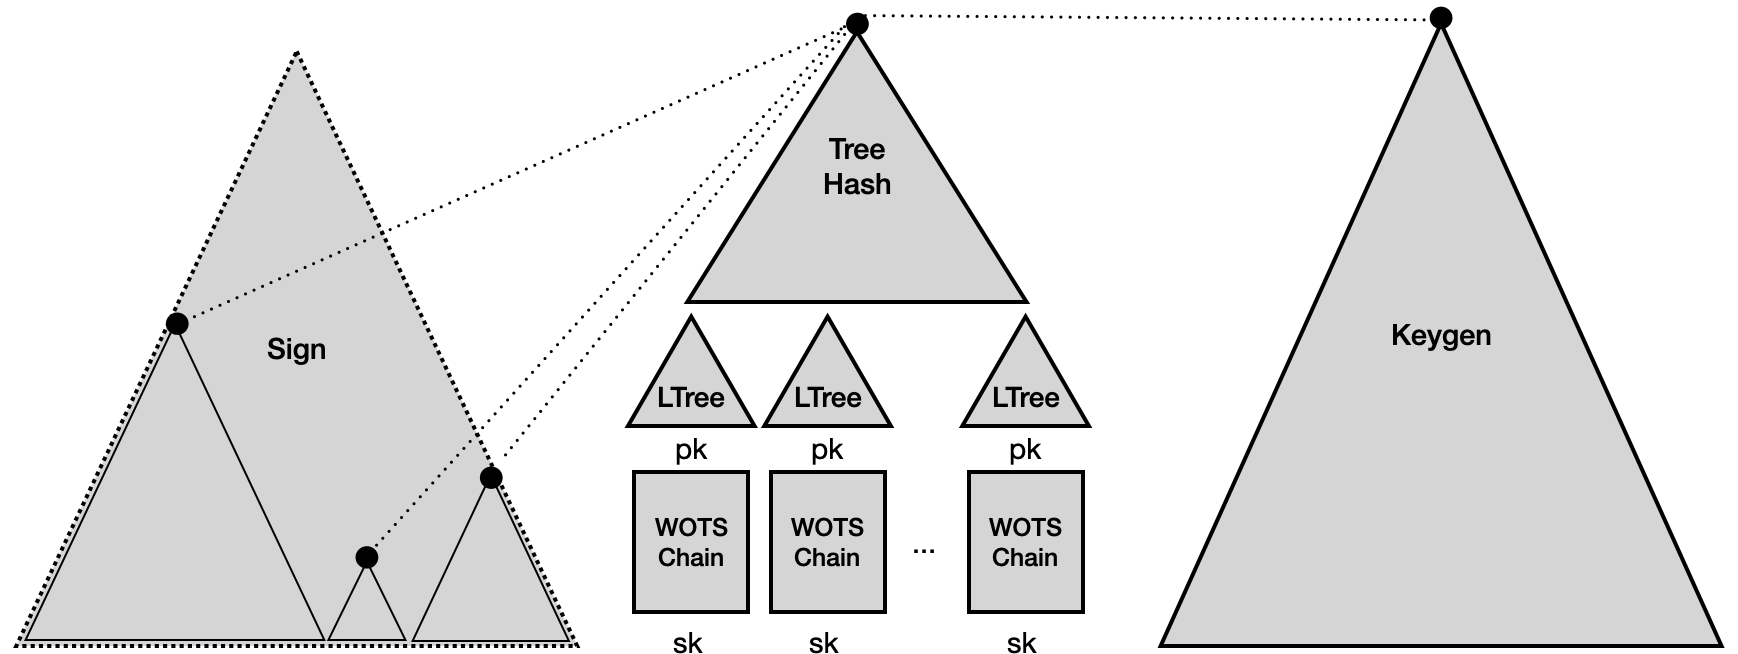
\includegraphics[width=\linewidth]{img/treehash.png}
\end{column}
\end{columns}
\end{frame}


\begin{frame}[plain]
  \centering
  {\usebeamerfont{title}\color{Teal}QUESTIONS?}
\end{frame}

\begin{frame}[allowframebreaks]{References}
  \footnotesize
  \setbeamertemplate{bibliography item}[text]
  \bibliographystyle{alpha}
  \bibliography{cryptobib/abbrev3,cryptobib/crypto,refs}
\end{frame}

\end{document}
